% =======================================================================================
\section{Background and Related Work}
\label{sec:background}
% =======================================================================================
% Brief by design: app:related is the long comparison.

% 2026-11-22 (user): Figure 2 placed here so that it lands on page 3.
\begin{figure*}[t]
  \centering
  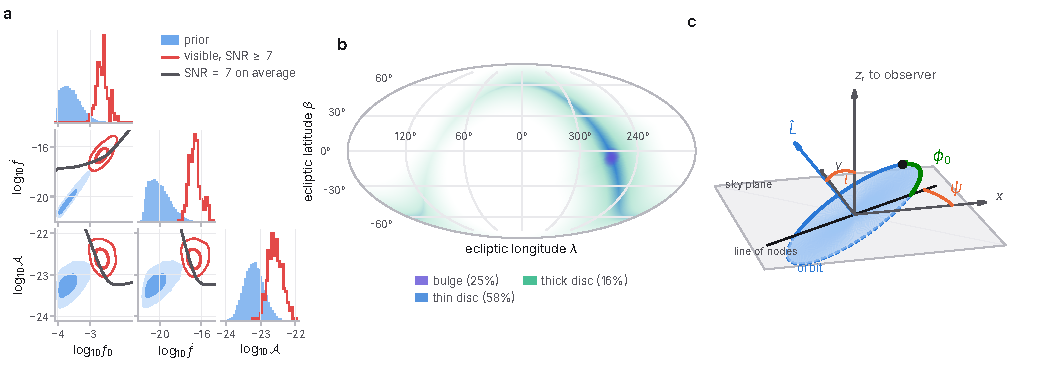
\includegraphics[width=\textwidth]{figures/priors.pdf}
  \caption{A visual representation of the \ac{gb} parameters and their priors. (a)~$(\log_{10}f_0, \log_{10}\fdot, \log_{10}\Amp)$ over the full band,
  \num{\ChartPriorDraws} sources in windows centred on the catalogue's $f_0$ marginal: regions
  enclosing \qty{\PriorCornerInner}{\percent} and \qty{\PriorCornerOuter}{\percent} of the prior
  (blue) and of the sources with $\snr\ge\PriorsVisibleSnr$ (red), and the line
  $\snr=\PriorsVisibleSnr$ (grey), which averages over the other parameters, so sources
  that reach it through a favourable sky or orientation also lie below it. (b)~The sky,
  \cref{eq:priors-sky}, in ecliptic coordinates $(\lambda, \beta)$: the bulge, the thick and the thin
  disc. (c)~The orientation: the orbit (blue, dashed
  below the sky plane) is inclined by $\iota$ to the sky plane $(x, y)$, with $z$ towards the observer; its line of nodes
  (black, dashed) is at $\psi$ from $x$, and $\phi_0$ is the phase along the orbit at the start of the observation.}
  \label{fig:priors}
\end{figure*}

\paragraph{The global fit.}
\label{sec:background-gw}\label{sec:gw-globalfit}
The \ac{lisa} data hold every source at once, so they are analysed by a global fit: a
reversible-jump \ac{mcmc} \citep{green1995reversible} over the sources of all kinds, their number
and the noise
\citep{cornish2005lisa,littenberg2020global,littenberg2023prototype,katz2024efficient,strub2024global,deng2025modular}.
On a simulated year of data, current pipelines return \numrange{5000}{12000} \acp{gb} for \num{700}
to about $10^6$ \ac{cpu} hours, and every new dataset or change of model pays that cost again
(\cref{tab:gw-globalfit}, \cref{app:related-globalfit}).

\paragraph{Simulation-based inference.}
\label{sec:inversion}\label{sec:background-generative}
Given data $d$, a prior $\pi(\theta)$ and a likelihood $p(d\mid\theta)$, the posterior is
$p(\theta\mid d)\propto p(d\mid\theta)\,\pi(\theta)$. Samplers such as \ac{mcmc} and nested
sampling \citep{skilling2006nested} evaluate the likelihood many times and start again for every
dataset. \Ac{sbi} \citep{cranmer2020frontier} instead trains a conditional density
estimator on simulated pairs $(\theta,d)$; in \ac{npe} the estimator models the posterior itself
\citep{papamakarios2016fast,greenberg2019automatic}. Training needs only a simulator, and the
posterior of a new dataset costs only network evaluations, but nothing guarantees the estimate. It
is checked with rank statistics over many simulations, \ac{sbc} \citep{talts2018validating} and
\ac{tarp} \citep{lemos2023sampling}, which are necessary conditions only (\cref{sec:validation}).

Flow matching, rectified flows and stochastic interpolants
\citep{lipman2023flow,liu2023flow,albergo2023building} train a generative model by regression: a
network learns the velocity that carries a simple base distribution to the data along prescribed
paths, and a sample solves an ordinary differential equation. Its quality depends on what the
network predicts, how the loss is weighted along the path and how the sampler spaces its steps
\citep{karras2022elucidating,kingma2023understanding}. For posteriors it entered \acs{sbi}
as \ac{fmpe} \citep{dax2023flow}. A posterior differs from an image in that its width
matters and can be orders of magnitude below the prior's, which is where our objective departs from
standard \ac{fmpe} (\cref{sec:method-fm}). Our network is a \ac{mmdit}
\citep{peebles2023scalable,esser2024scaling} with the data and the sources as its two streams
(\cref{sec:method-network}).

\paragraph{\Acs{sbi} for gravitational waves.}
\label{sec:background-gw-npe}\label{sec:background-gb}
\Acs{sbi} is established for the compact binaries of ground-based detectors
\citep{green2020gravitational,gabbard2022bayesian,dax2021real,dax2025real}, with importance sampling to
the exact posterior \citep{dax2023neural}, and for \ac{lisa}'s massive black-hole binaries
\citep{du2024advancing,liang2024rapid,spadaro2026accurate}. Overlapping signals have been analysed
jointly a pair at a time on the ground \citep{langendorff2023normalizing,papalini2025can}. For
\acp{gb}, normalising flows serve inside the global fit as priors and proposals fitted to one
source's chains \citep{korsakova2024neural}. As posterior estimators, \citet{delmond2026neural}
train a neural spline flow on one \ac{gb} under the full response and, as a proof of concept, on
two; \citet{mao2025robust} apply \ac{fmpe} to one source with three free parameters in gapped data;
and SlotFlow \citep{houba2025slotflow} infers up to ten sinusoids in white noise, with a posterior
that factorises over its slots. None returns a joint posterior over more than two sources under the
\ac{lisa} response (\cref{app:related}).
